\subsection{Image\-Gtransfo  Class Reference}
\label{class_imagegtransfo}\index{ImageGtransfo@{Image\-Gtransfo}}
{\tt \#include $<$transformedimage.h$>$}

Inheritance diagram for Image\-Gtransfo::\begin{figure}[H]
\begin{center}
\leavevmode
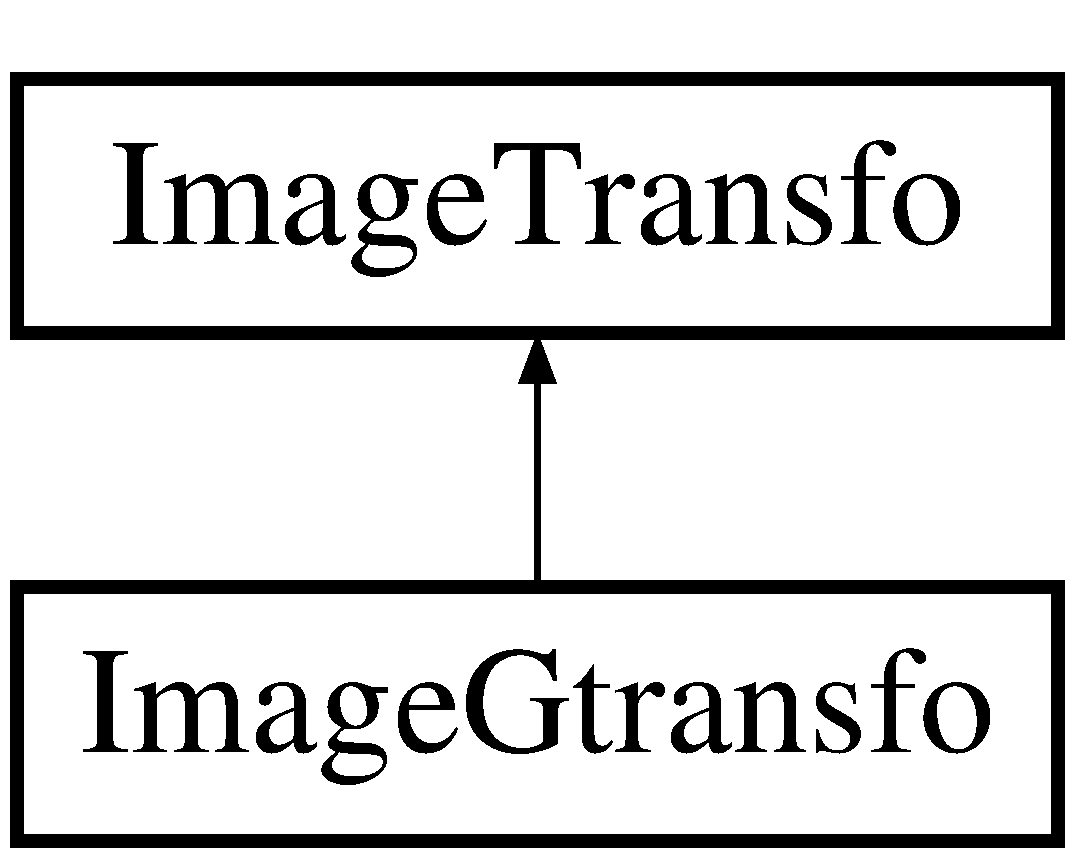
\includegraphics[height=2cm]{class_imagegtransfo}
\end{center}
\end{figure}
\subsubsection*{Public Methods}
\begin{CompactItemize}
\item 
\index{ImageGtransfo@{ImageGtransfo}!ImageGtransfo@{Image\-Gtransfo}}\index{ImageGtransfo@{ImageGtransfo}!ImageGtransfo@{Image\-Gtransfo}}
{\bf Image\-Gtransfo} (const {\bf Gtransfo} $\ast$Transfo\-From\-Ref, const {\bf Gtransfo} $\ast$Transfo\-To\-Ref, const {\bf Frame} \&Output\-Image\-Size, const string \&Geom\-Ref\-Name)\label{class_imagegtransfo_a0}

\item 
\index{ImageGtransfo@{ImageGtransfo}!ImageGtransfo@{Image\-Gtransfo}}\index{ImageGtransfo@{ImageGtransfo}!ImageGtransfo@{Image\-Gtransfo}}
{\bf Image\-Gtransfo} (const {\bf Reduced\-Image} \&Ref, const {\bf Reduced\-Image} \&To\-Align)\label{class_imagegtransfo_a1}

\begin{CompactList}\small\item\em the output image size is the one of the Ref. Finds the transfo(s).\item\end{CompactList}\item 
\index{ImageGtransfo@{ImageGtransfo}!ImageGtransfo@{Image\-Gtransfo}}\index{ImageGtransfo@{ImageGtransfo}!ImageGtransfo@{Image\-Gtransfo}}
{\bf Image\-Gtransfo} ()\label{class_imagegtransfo_a2}

\item 
\index{TransfoFromRef@{TransfoFromRef}!ImageGtransfo@{Image\-Gtransfo}}\index{ImageGtransfo@{ImageGtransfo}!TransfoFromRef@{Transfo\-From\-Ref}}
{\bf Gtransfo}$\ast$ {\bf Transfo\-From\-Ref} () const\label{class_imagegtransfo_a3}

\item 
\index{TransfoToRef@{TransfoToRef}!ImageGtransfo@{Image\-Gtransfo}}\index{ImageGtransfo@{ImageGtransfo}!TransfoToRef@{Transfo\-To\-Ref}}
{\bf Gtransfo}$\ast$ {\bf Transfo\-To\-Ref} () const\label{class_imagegtransfo_a4}

\item 
\index{FromRef@{FromRef}!ImageGtransfo@{Image\-Gtransfo}}\index{ImageGtransfo@{ImageGtransfo}!FromRef@{From\-Ref}}
const {\bf Gtransfo}$\ast$ {\bf From\-Ref} () const\label{class_imagegtransfo_a5}

\item 
\index{GeomRefName@{GeomRefName}!ImageGtransfo@{Image\-Gtransfo}}\index{ImageGtransfo@{ImageGtransfo}!GeomRefName@{Geom\-Ref\-Name}}
string {\bf Geom\-Ref\-Name} () const\label{class_imagegtransfo_a6}

\item 
\index{dump@{dump}!ImageGtransfo@{Image\-Gtransfo}}\index{ImageGtransfo@{ImageGtransfo}!dump@{dump}}
virtual void {\bf dump} (ostream \&s=cout)\label{class_imagegtransfo_a7}

\item 
\index{TransformImage@{TransformImage}!ImageGtransfo@{Image\-Gtransfo}}\index{ImageGtransfo@{ImageGtransfo}!TransformImage@{Transform\-Image}}
void {\bf Transform\-Image} (const {\bf Fits\-Image} \&Source, {\bf Fits\-Image} \&Transformed, const {\bf Reduced\-Image} $\ast$Source, {\bf Reduced\-Image} $\ast$Result, double Default\-Val=0) const\label{class_imagegtransfo_a8}

\begin{CompactList}\small\item\em the one that transforms the image and update header.\item\end{CompactList}\item 
\index{TransformWeightImage@{TransformWeightImage}!ImageGtransfo@{Image\-Gtransfo}}\index{ImageGtransfo@{ImageGtransfo}!TransformWeightImage@{Transform\-Weight\-Image}}
void {\bf Transform\-Weight\-Image} (const {\bf Fits\-Image} \&Source, {\bf Fits\-Image} \&Transformed) const\label{class_imagegtransfo_a9}

\begin{CompactList}\small\item\em Transforms a weight image.\item\end{CompactList}\item 
\index{TransformBoolImage@{TransformBoolImage}!ImageGtransfo@{Image\-Gtransfo}}\index{ImageGtransfo@{ImageGtransfo}!TransformBoolImage@{Transform\-Bool\-Image}}
void {\bf Transform\-Bool\-Image} (const {\bf Fits\-Image} \&Source, {\bf Fits\-Image} \&Transformed) const\label{class_imagegtransfo_a10}

\begin{CompactList}\small\item\em transforms a bool {\bf Image} {\rm (p.\,\pageref{class_image})}.\item\end{CompactList}\item 
\index{TransformCatalog@{TransformCatalog}!ImageGtransfo@{Image\-Gtransfo}}\index{ImageGtransfo@{ImageGtransfo}!TransformCatalog@{Transform\-Catalog}}
void {\bf Transform\-Catalog} (const {\bf SEStar\-List} \&Catalog, {\bf SEStar\-List} \&Transformed) const\label{class_imagegtransfo_a11}

\item 
\index{IsValid@{IsValid}!ImageGtransfo@{Image\-Gtransfo}}\index{ImageGtransfo@{ImageGtransfo}!IsValid@{Is\-Valid}}
bool {\bf Is\-Valid} () const\label{class_imagegtransfo_a12}

\item 
\index{ScaleFactor@{ScaleFactor}!ImageGtransfo@{Image\-Gtransfo}}\index{ImageGtransfo@{ImageGtransfo}!ScaleFactor@{Scale\-Factor}}
double {\bf Scale\-Factor} () const\label{class_imagegtransfo_a13}

\item 
\index{Clone@{Clone}!ImageGtransfo@{Image\-Gtransfo}}\index{ImageGtransfo@{ImageGtransfo}!Clone@{Clone}}
Image\-Transfo$\ast$ {\bf Clone} () const\label{class_imagegtransfo_a14}

\item 
\index{~ImageGtransfo@{$\sim$ImageGtransfo}!ImageGtransfo@{Image\-Gtransfo}}\index{ImageGtransfo@{ImageGtransfo}!~ImageGtransfo@{$\sim$Image\-Gtransfo}}
{\bf $\sim$Image\-Gtransfo} ()\label{class_imagegtransfo_a15}

\end{CompactItemize}


\subsubsection{Detailed Description}
geometric transfo of a reduced image. 



The documentation for this class was generated from the following file:\begin{CompactItemize}
\item 
{\bf transformedimage.h}\end{CompactItemize}
